{
\renewcommand{\baselinestretch}{1.0}
\begin{figure}[t]
\begin{center}

%\resizebox{\columnwidth}{!} {
%   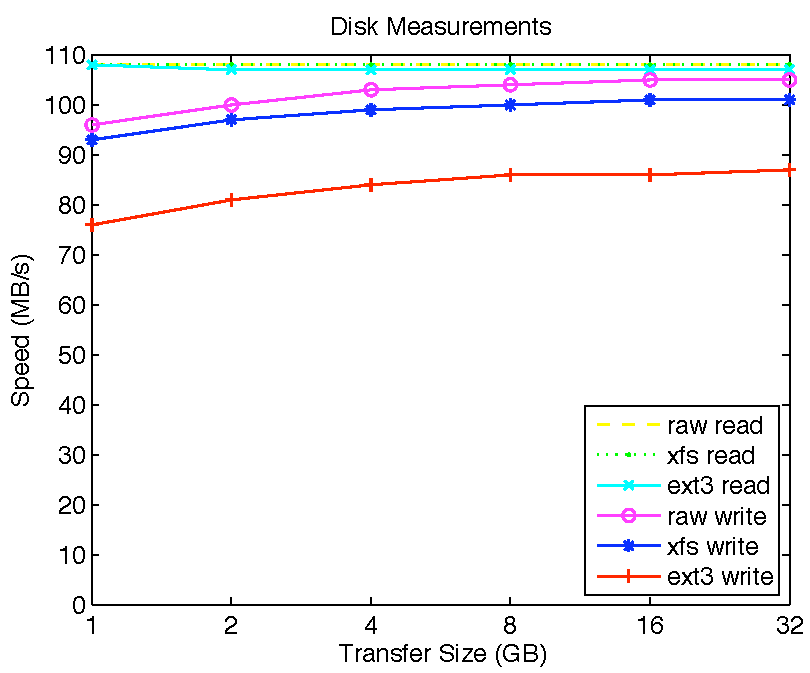
\includegraphics[height=2.5in]{fig_disk_measurements.pdf}
   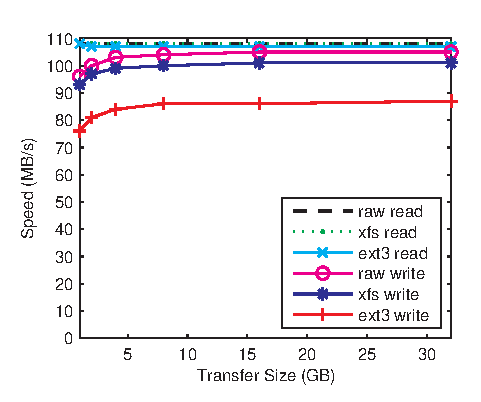
\includegraphics[height=2.5in]{fig_disk_measurements.eps}
%  }

\end{center}
\minicaption{Disk read and write measurements for a Seagate Barracuda drive}
{While read performance is consistently high across all systems,
  writes are slower, and \texttt{ext3} writes in particular are around
  20\% slower than raw device writes.}  

\label{fig:disk_measurements}
\end{figure}
}

